\section{采样接口}\label{sec:采样接口}
正如先在\refsub{应用到图像合成}介绍的,
pbrt中实现的渲染方法包含了在图像平面的2D点之外的额外维度上选择样本点。
各种算法将用于生成这些点,但它们的所有实现都继承自定义其接口的抽象类\refvar{Sampler}{}。
核心采样声明和函数在文件\href{https://github.com/mmp/pbrt-v3/blob/master/src/core/sampler.h}{\ttfamily core/sampler.h}
和\href{https://github.com/mmp/pbrt-v3/blob/master/src/core/sampler.cpp}{\ttfamily core/sampler.cpp}中。
样本生成的每种实现都在目录{\ttfamily samplers/}下其自己的源文件内。

\refvar{Sampler}{}的任务是生成$[0,1)^n$中$n$维样本的序列,
其中每个图像样本都要为其生成这样的样本向量,且每个样本中的维数$n$可能会变,
这取决于光传输算法执行的计算(见\reffig{7.13})。
\begin{figure}[htbp]
    \centering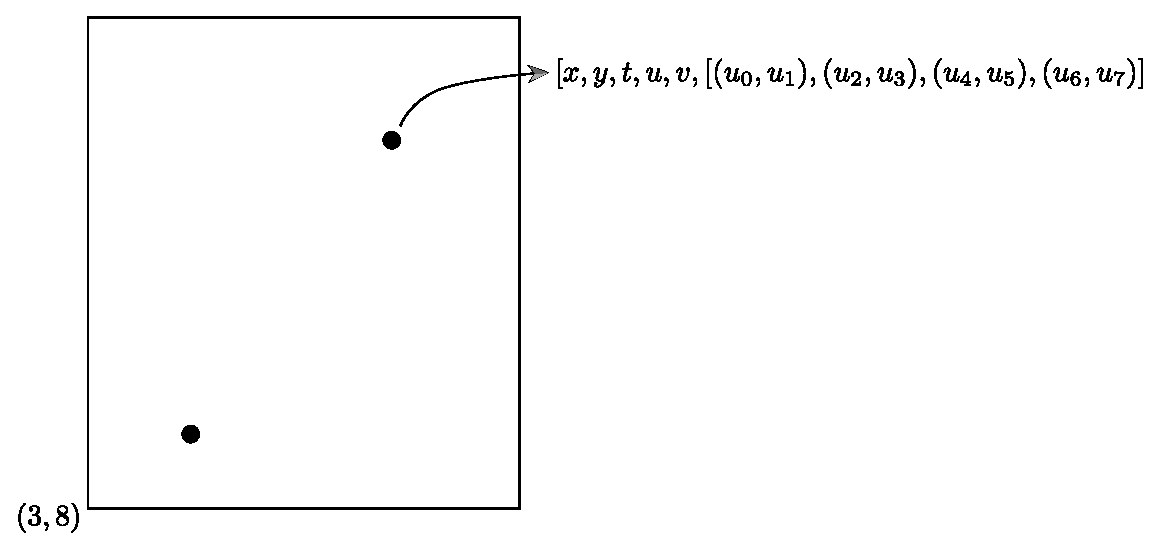
\includegraphics[width=0.9\linewidth]{chap07/Samplerndimensional.eps}
    \caption{采样器为每个图像样本生成用来合成最终图像的$n$维样本向量。
        这里,像素$(3,8)$正被采样,且在该像素区域内有两个图像样本。
        样本向量的前两维给出样本在该像素内的偏移量$(x,y)$,
        接下来三维决定相应相机光线的时间和透镜位置。后续维度用于
        第\refchap{光传输I:表面反射}、\refchap{光传输II:体积渲染}和\refchap{光传输III:双向方法}中
        的蒙特卡洛光传输算法。这里,光传输算法已经请求了样本向量中的四个2D数组样本;
        例如,这些值可能用于选择面光源上的四个点来为图像样本计算辐亮度。}
    \label{fig:7.13}
\end{figure}

因为样本值必须严格小于1,所以定义一个常数\refvar{OneMinusEpsilon}{}很有用,
它表示小于1的最大可表示浮点常数。然后,我们会截断样本向量值使之不大于该值。
\begin{lstlisting}
`\initcode{Random Number Declarations}{=}`
#ifdef PBRT_FLOAT_IS_DOUBLE
static const `\refvar{Float}{}` `\initvar{OneMinusEpsilon}{}` = 0x1.fffffffffffffp-1;
#else
static const `\refvar{Float}{}` OneMinusEpsilon = 0x1.fffffep-1;
#endif
\end{lstlisting}

可能最简单的\refvar{Sampler}{}实现是当每次需要样本向量的额外分量时直接返回$[0,1)$内的均匀随机值。
这样的采样器可产生正确的图像但会需要非常多的样本(以及更多要追踪的光线与更多的时间)来
创建用更先进采样器所能取得的相同质量的图像。
使用更佳采样模式的运行时间开销大致和用诸如均匀随机数的低质量模式相同;
因为为每个图像样本计算辐亮度比计算样本的分量值会有大得多的开销,
所以这样做是有回报的(\reffig{7.14})。
\begin{figure}[htbp]
    \centering
    \subfloat[差的采样]{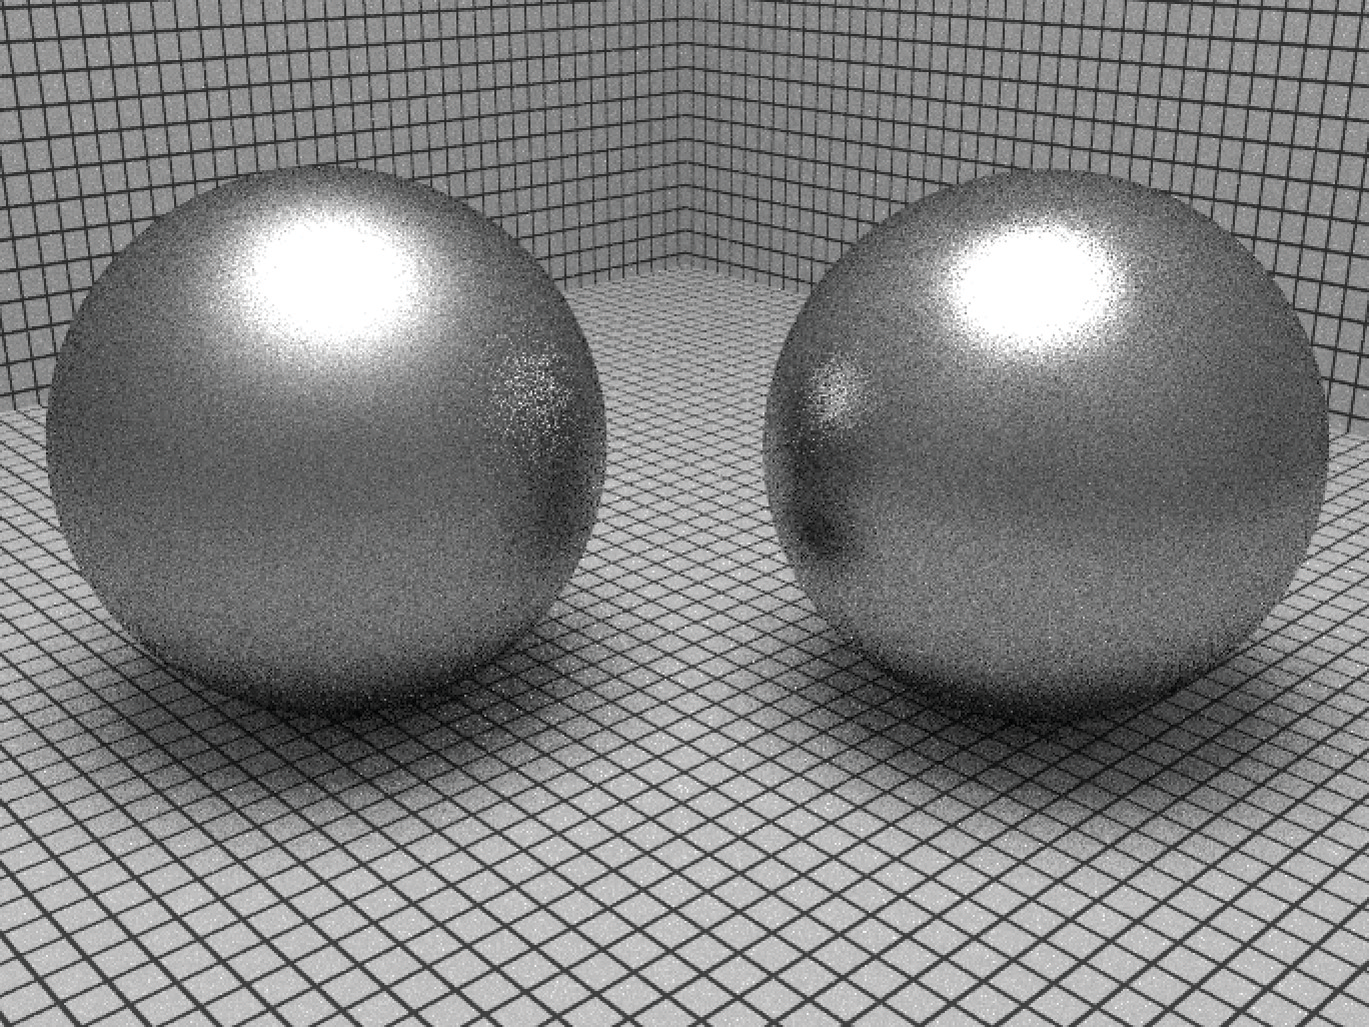
\includegraphics[width=\linewidth]{chap07/spheres-bad-sampler.png}\label{fig:7.14.1}}\\
    \subfloat[更好的采样]{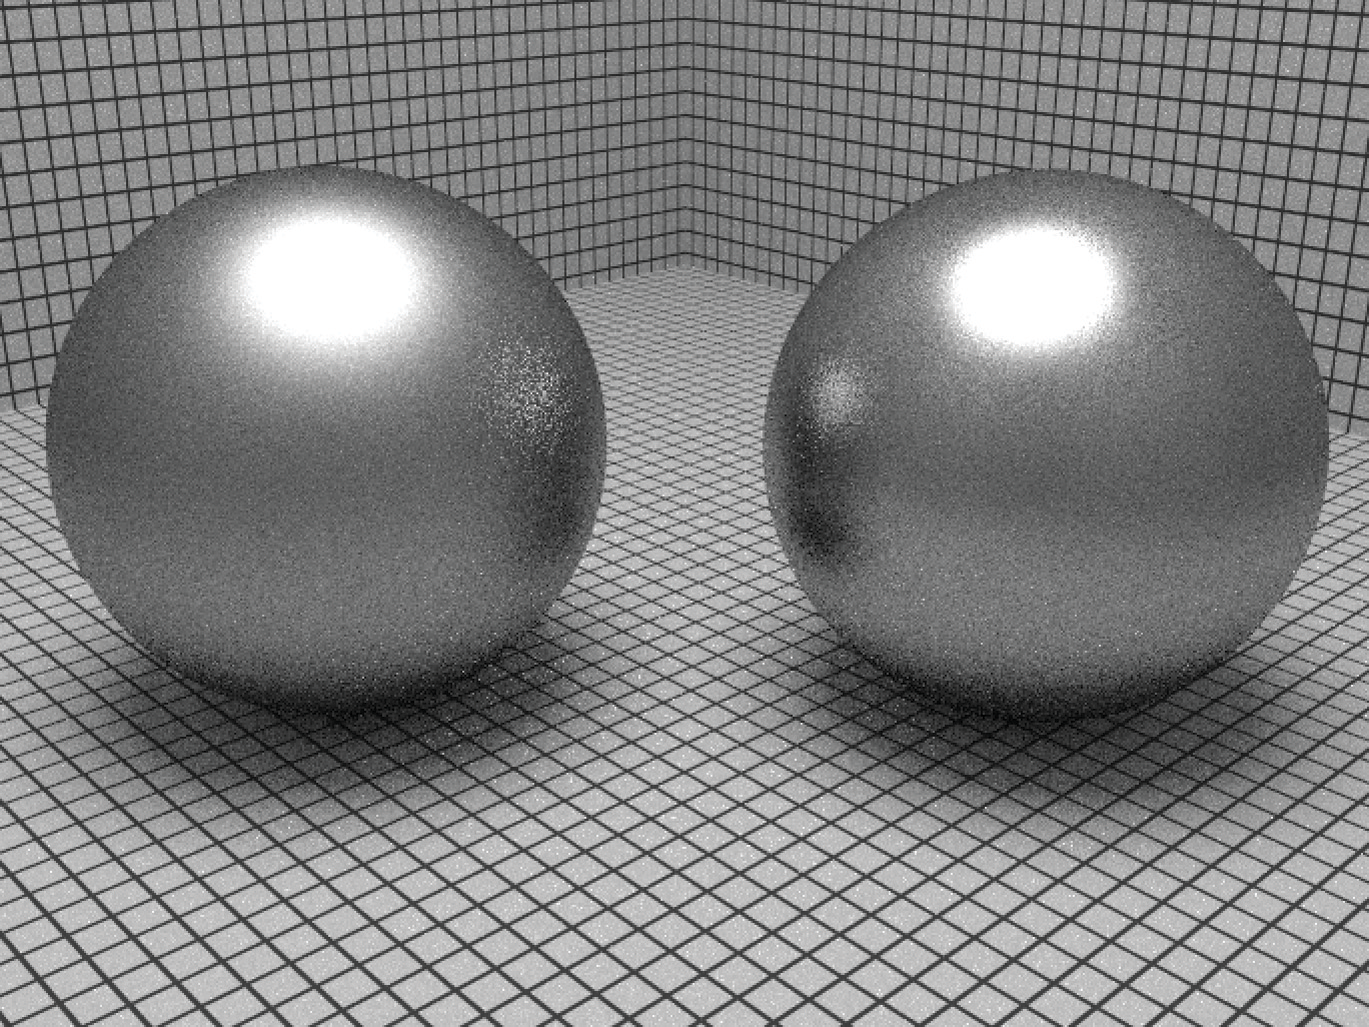
\includegraphics[width=\linewidth]{chap07/spheres-better-sampler.png}\label{fig:7.14.2}}
    \caption{用(a)相对低效的采样器和(b)精心设计的采样器渲染的场景,
        它们用了同样多的样本。从高光边缘到光泽反射,图像质量的提升是明显的。}
    \label{fig:7.14}
\end{figure}

下面假设这些样本向量的一些特性:
\begin{itemize}
    \item \refvar{Sampler}{}生成的前五维通常由\refvar{Camera}{}使用。
    这种情况下,前两个专门用于选择图像上当前像素区域内的点;
    第三个用于计算应该取用该样本的时间;第四和五维为景深给出透镜位置$(u,v)$。
    \item 一些采样算法在样本向量的某些维度中生成的样本比其他维度更好。
    在系统其他地方,我们假设一般前面的维度具有放置得最好的样本值。
\end{itemize}

还要注意\refvar{Sampler}{}生成的$n$维样本通常不会整个显式表示或存储,
而是常常按照光传输算法的需要逐步生成。(然而,存储整个样本向量并对其分量逐渐作出调整
是\refsub{基本样本空间采样器}中\refvar{MLTSampler}{}的基础,
它用于\refsub{MLT积分器}的\refvar{MLTIntegrator}{}。)

\subsection{评估样本模式:差异}\label{sub:评价样本模式:差异}
\begin{remark}
    本节含有高级内容,第一次阅读时可以跳过。
\end{remark}

傅里叶分析给了我们一种方法来评估2D采样模式的质量,

\subsection{基本采样器接口}\label{sub:基本采样器接口}

\begin{lstlisting}
`\initcode{Sampler Declarations}{=}\initnext{SamplerDeclarations}`
class `\initvar{Sampler}{}` {
public:
    `\refcode{Sampler Interface}{}`
    `\refcode{Sampler Public Data}{}`
protected:
    `\refcode{Sampler Protected Data}{}`
private:
    `\refcode{Sampler Private Data}{}`
};
\end{lstlisting}
\begin{lstlisting}
`\initcode{Sampler Method Definitions}{=}\initnext{SamplerMethodDefinitions}`
`\refvar{Sampler}{}`::`\refvar{Sampler}{}`(int64_t samplesPerPixel)
: `\refvar{samplesPerPixel}{}`(samplesPerPixel) { }
\end{lstlisting}
\begin{lstlisting}
`\initcode{Sampler Public Data}{=}`
const int64_t `\initvar{samplesPerPixel}{}`;
\end{lstlisting}
\begin{lstlisting}
`\initcode{Sampler Interface}{=}\initnext{SamplerInterface}`
virtual void `\initvar{StartPixel}{}`(const `\refvar{Point2i}{}` &p);
\end{lstlisting}
\begin{lstlisting}
`\refcode{Sampler Interface}{+=}\lastnext{SamplerInterface}`
virtual `\refvar{Float}{}` `\initvar{Get1D}{}`() = 0;
virtual `\refvar{Point2f}{}` `\initvar{Get2D}{}`() = 0;
\end{lstlisting}
\begin{lstlisting}
`\refcode{Sampler Method Definitions}{+=}\lastnext{SamplerMethodDefinitions}`
`\refvar{CameraSample}{}` `\refvar{Sampler}{}`::`\initvar{GetCameraSample}{}`(const `\refvar{Point2i}{}` &pRaster) {
    `\refvar{CameraSample}{}` cs;
    cs.`\refvar{pFilm}{}` = (`\refvar{Point2f}{}`)pRaster + `\refvar{Get2D}{}`();
    cs.`\refvar[CameraSample::time]{time}{}` = `\refvar{Get1D}{}`();
    cs.`\refvar{pLens}{}` = `\refvar{Get2D}{}`();
    return cs;
}
\end{lstlisting}
\begin{lstlisting}
`\refcode{Sampler Interface}{+=}\lastnext{SamplerInterface}`
virtual bool `\initvar{StartNextSample}{}`();
\end{lstlisting}
\begin{lstlisting}
`\refcode{Sampler Interface}{+=}\lastnext{SamplerInterface}`
virtual std::unique_ptr<`\refvar{Sampler}{}`> `\initvar{Clone}{}`(int seed) = 0;
\end{lstlisting}